\chapter{基于带约束Delaunay triangulation的分治算法}

在论文编写期间,受分治Delaunay triangulation算法以及一些已有研究\upcite{chew1987constrained}的启发,我想到了另一种解决本问题的思路。

我们已知,Delaunay triangulation广泛被认为是三角剖分中的最优结果,其具有多种优良性质,如最小角最大,局部修改只影响小范围区域等。
而在三角剖分中,我们能够产生选择的最小单位如图\ref*{basecell}所示,是一个包含四个点的凸多边形。根据内部两条对角线的选择方式,有着两种不同的分割结果。标准的Delaunay Triangulation根据三角形外接圆相关的信息用于评估两条边的选择,而两条对角线的选择可以在不影响四边形外部的情况下进行切换。

\begin{figure}[htp]
    \centering
    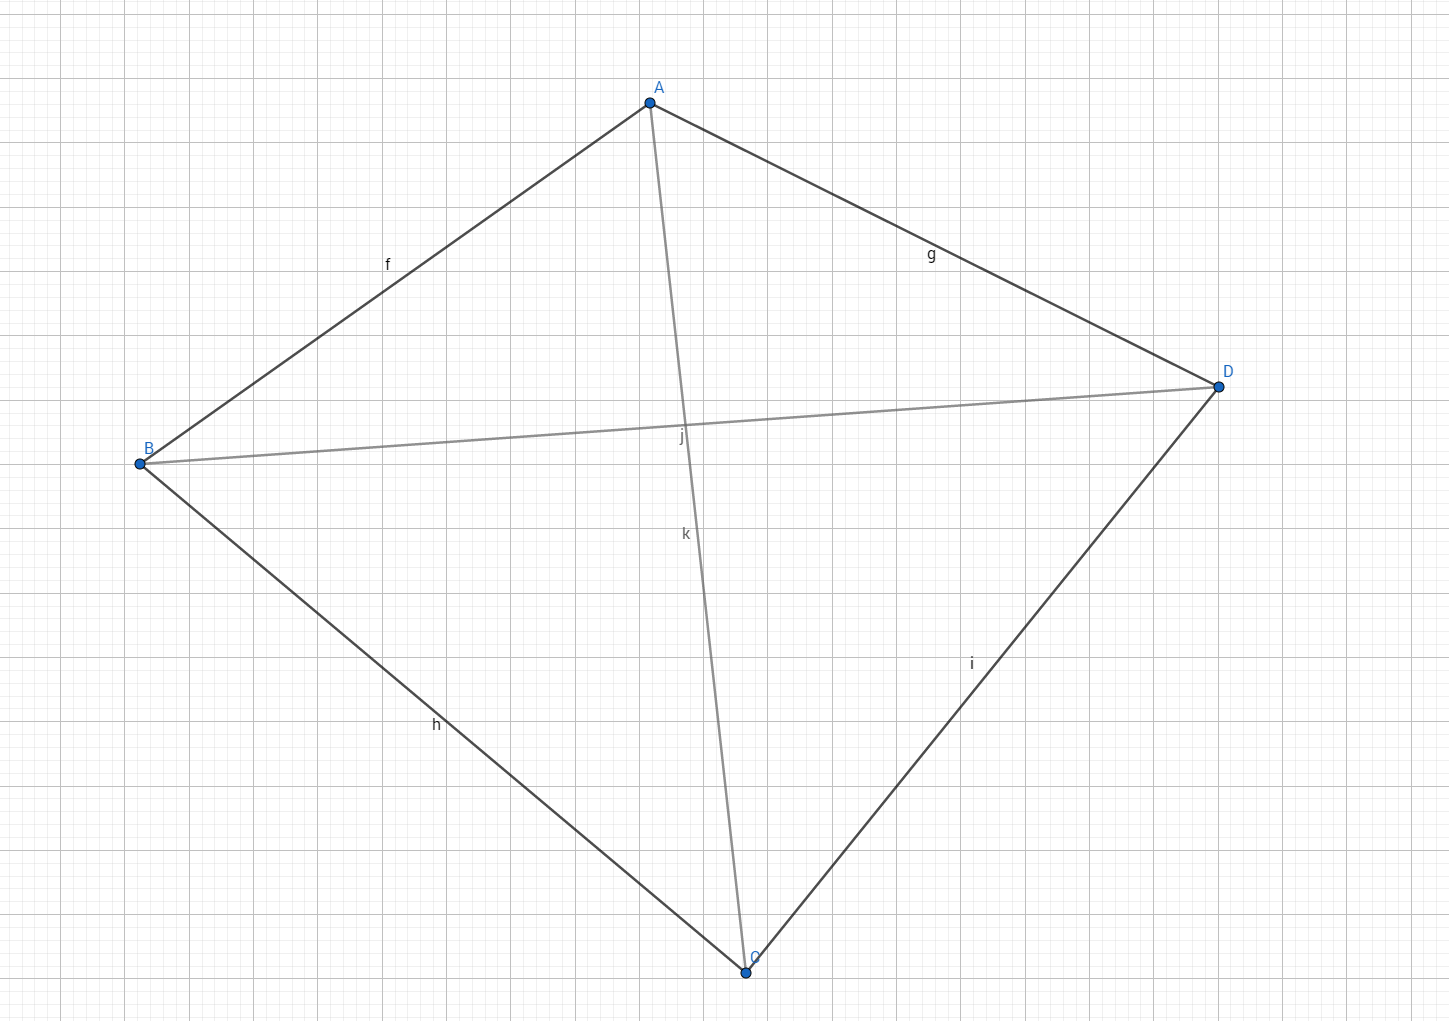
\includegraphics[width=0.5\textwidth]
    {figures/basecell.png}
    \caption{三角剖分中的最小单位}
    \label{basecell}
  \end{figure}

从另一个角度来看,对于一个完成剖分后的三角网,除去外边界以外的边,所有的边都恰好包含于两个三角形,而这两个三角形可能会组成上述的凸四边形。
在这种情况下,我们可以对这条边,以及这条边所对应的四边形的另一条对角线进行一次“交换”,在仅有小范围改动的情况下对三角剖分进行修正。

由此我们可以考虑一种思路,即在点集的Delaunay三角网中,强行加入原多边形已有的边作为限制,并在改动尽量小的情况下维持答案为合法的三角剖分。

此算法要求存在包含全部原多边形边的合法三角网,即原多边形的边不能相交。因此无法用于复杂多边形,但复杂多边形可以通过一定的预处理后变为可以执行本算法的状态。

\section{用于生成基础三角网的分治delaunay算法}
使用分治算法生成Delaunay三角网的步骤不再赘述。不过,为了便于后续计算,我们采用与之前不同的数据结构用于存储信息。

我们采用数组记录整个多边形的点集,并分别对每个顶点按极角序记录其在三角网中的连边。

计算完Delaunay三角网后,我们便获得了一份初始的三角剖分结果。这份剖分结果中不包含原多边形连边的信息,是接下来计算答案的基础。
\section{基于交换操作的约束边加入方法}
在本节中,我们将原多边形的每一条边强制加入Delaunay三角网。在一条边的加入期间,我们最终将会删除所有与之冲突的边,并补充一定数量的次优边以保持三角网的性质。

下面,我们选择一条边,开始将其加入Delaunay三角网中。

\begin{figure}[htp]
    \centering
    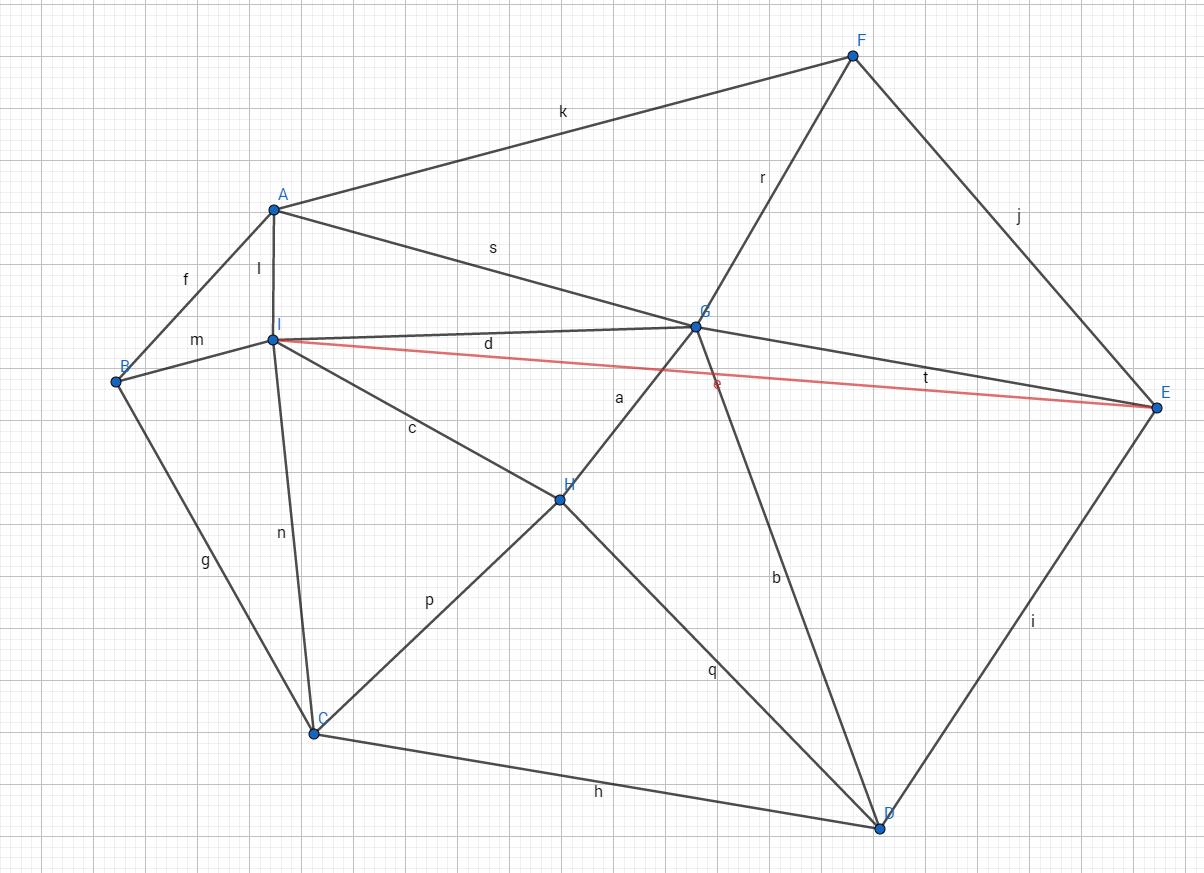
\includegraphics[width=0.5\textwidth]
    {figures/addconstrant.png}
    \caption{向三角网中强制加入限制边}
    \label{addedge}
  \end{figure}

一种最简单的情况是,当前的边已经被原三角网所包含。在这种情况下,我们不需要对原三角网进行修改,只需要标注当前边属于不可移除的限制边即可。

另一种情况下,当前边的加入仅涉及了两个三角形,也就是上文中图\ref*{basecell}的情况,存在两条冲突的”对角线“,代表我们在当前四边形的剖分结果中需要强制选择相对较差的结果。
也就是说明,此时在四边形对角线的二选一中需要进行一次“交换”操作,即可完成对三角网的修正。

最后一种情况则是,新增的连边破坏了多个三角网。如图\ref*{addedge}所示,新加入的红色边与多条已有的边相冲突。在这种情况下,我们只需依次处理每条与新增边冲突的旧边即可。
我们按冲突点顺序遍历所有的冲突边。对于一条冲突边,我们可以寻找这条边对应的两个三角形,并对其尝试进行一次“交换”操作。在进行两次”交换“后,如图\ref*{swap}所示,我们成功将新的限制边加入了三角网中。

\begin{figure}[htp]
    \centering
    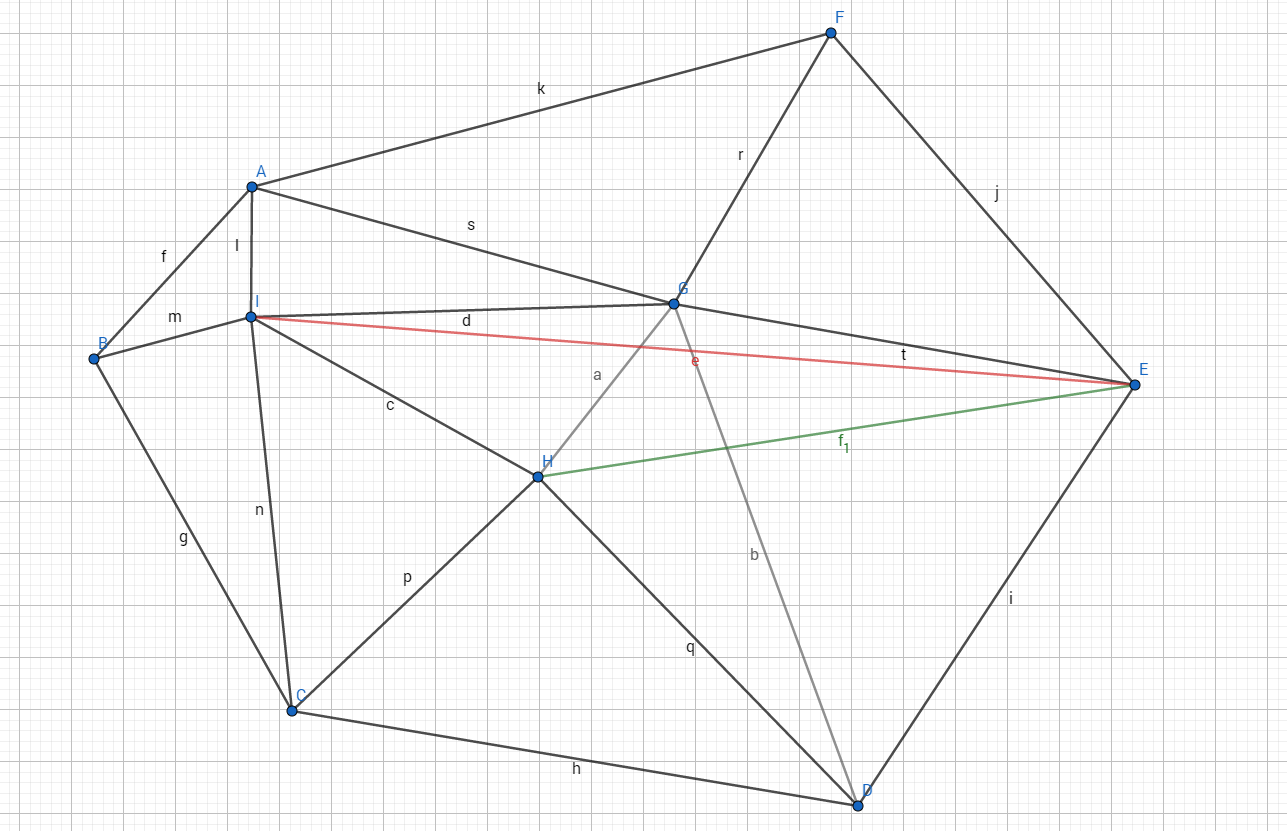
\includegraphics[width=0.5\textwidth]
    {figures/swap.png}
    \caption{通过交换操作修正三角网使其满足要求}
    \label{swap}
  \end{figure}

若两个三角形组成的四边形为凸四边形,且四边形有三个点在新增边同侧或为新增边端点,则“交换”操作结束后即可消除一条冲突边。
若组成的四边形为凹四边形,无法执行“交换”操作,我们暂时跳过该点,在后续操作中将其完成消除。

如图所示,我们以新增边的顶点之一为起点,向另一个顶点在新增边的两侧各连接一条最贴近新增边的折线。
该折线满足性质,从折线中间某条边向新增边方向搜索,下一条边必为冲突边。
两条折线产生了一个包含新增边的多边形,且多边形内部仅存在冲突边,所有冲突边均在多边形内。
易证这样的折线在新增边的两侧有且仅有一条。

将可以直接执行“交换”操作的边处理完后,有较小的概率仍存在未被消除的冲突边。如图\ref*{deadlock}所示,此种情况下多边形不存在可以进行交换的边。此时我们选择冲突边中最长的一条,对其进行一次“交换”操作。操作结束后,根据李立新的证明\upcite{李立新1999约束},必然存在了新的可消除冲突边。多次处理后我们最终可以对全部冲突边进行消除,并成功将新增边强制加入三角剖分结果作为约束。

\begin{figure}[htp]
    \centering
    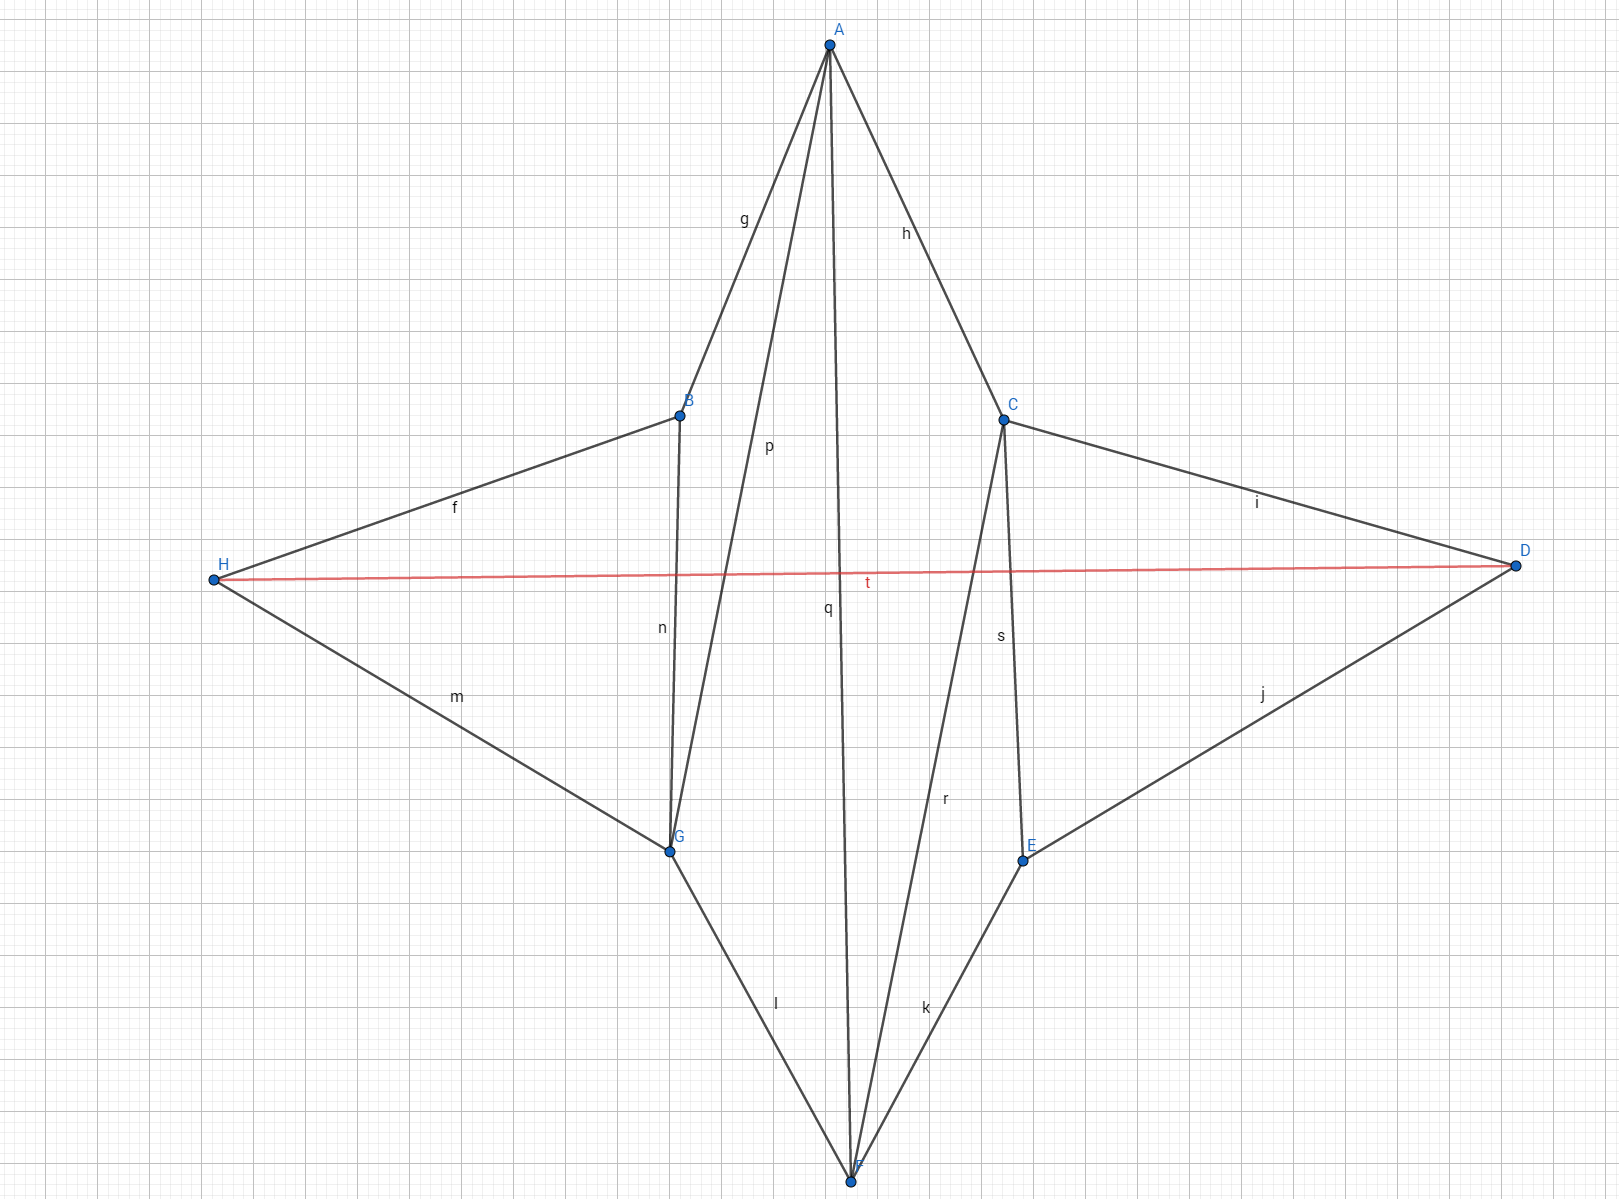
\includegraphics[width=0.5\textwidth]
    {figures/deadlock.png}
    \caption{不存在可以直接通过交换消除的冲突边的特殊情况}
    \label{deadlock}
  \end{figure}

由此,我们可以构建一个包含原多边形中全部连边的点集三角剖分结果。

\section{基于边与多边形关系生成三角剖分解}

从之前对点集的三角划分到最终多边形三角剖分的结果仍存在一定的距离。
完成点集的三角剖分结果计算后,剖分结果所形成的多边形是包含原多边形所有节点的凸包。我们需要从剖分结果中去除不属于原多边形的部分,保留的部分即为三角剖分的答案。

我们采用如下方法删除不属于原多边形的连边。

首先通过预处理判断多边形中每条边界的性质,确认边界包围的区间是否属于多边形;同时标准化多边形的旋转方向,使多边形的外边界为顺时针旋转,而孔洞的边界则为逆时针旋转。在此基础上,计算出每个顶点中连边所对应角度中属于多边形内部的范围。

枚举剖分结果中的连边。对于每条待判断边,任选一顶点。判断当前边是否落在顶点所对应的多边形顶角内部。若边落在多边形外部,则说明当前边不属于多边形三角划分的一部分,将其从最终结果中删除。

由此,我们便可以得到原多边形的三角剖分结果。